\documentclass[a4paper]{article}

%% Language and font encodings
\usepackage[english]{babel}
\usepackage[utf8x]{inputenc}
\usepackage[T1]{fontenc}

%% Sets page size and margins
\usepackage[a4paper,top=3cm,bottom=2cm,left=3cm,right=3cm,marginparwidth=1.75cm]{geometry}

%% Useful packages
\usepackage{amsmath}
\usepackage{graphicx}
\usepackage[colorinlistoftodos]{todonotes}
\usepackage[colorlinks=true, allcolors=blue]{hyperref}

\usepackage{caption}
\usepackage{subcaption}

\graphicspath{{res/}}

\title{Your Paper}
\author{Lukas Finkbeiner}

\begin{document}
\maketitle

\begin{abstract}

We studied signals.

\end{abstract}

% No need to re-derive anything!!

\section{Introduction and Background}

\subsection{The Fourier Transform}

Where $V(t)$ is voltage as a function of time and $V(\nu)$ is voltage as a function of frequency $\nu$.

\

$V(\nu) = \int_{-T / 2}^{T / 2} V(t) \exp(2 \pi i \nu t) dt$

\

Where T is the length of the time sample.

\

$V(t) = \frac{1}{\nu_s} \int_{- \nu_s / 2}^{\nu_s / 2} \tilde{V}(\nu) \exp(-2 \pi i \nu t) d \nu$

\

where $\nu_s$ is the sampling frequency used.

\textcolor{red}{What happens if you change the bounds in the manner (N / 2 - 1) / $\nu_s$}

% ?? I need to talk about Parseval's Theorem

\subsection{Positive and Negative Frequencies}

``complex inputs to a Fourier Transform break the positive/negative frequency degeneracy''

The sine function is odd:

$\sin(-\omega t) = -sin(\omega t)$

The cosine function is even:

$\cos(-\omega t) = \cos (\omega t)$

We can generalize under Euler's identity:

$A\exp(i \omega t) = A \cos(\omega t) + i \cdot A \sin(\omega t)$

$A\exp(-i \omega t) = A \cos(-\omega t) + i \cdot A \sin(-\omega t) = A \cos(\omega t) - i \cdot A \sin(\omega t)$

\subsection{Nyquist's Theorem and Aliasing}

$f_s > 2 f_{max}$

\subsection{The Convolution and Correlation Theorems}

The convolution of two functions $f(t)$ and $g(t)$ is defined as:

\

$[f * g](\tau) = \int_{-T / 2}^{T / 2} f(t) g(\tau - t) dt$

\

The correlation of two functions $f(t)$ and $g(t)$ is defined as

\

$[f \star g](\tau) = \int_{-T / 2}^{T / 2} f(t) g(\tau + t) dt$

\

\textcolor{red}{You may want to prove this by substituting the Fourier transform}

\

$[\tilde{f * g}](\nu) \equiv \int_{-T / 2}^{T / 2}[f * g](\tau) \exp{2 \pi i \tau \nu} d \tau = \tilde{f}(\nu) \cdot \tilde{g}(\nu)$

\

$[\tilde{f \star g}](\nu) \equiv \int_{-T / 2}^{T / 2}[f \star g](\tau) \exp{2 \pi i \tau \nu} d \tau = \tilde{f}(\nu) \cdot \tilde{g^*}(\nu)$

\textcolor{red}{Now: how is the ACF relevant to this paper}

\subsection{Sideband Theory}

All that sweet, sweet trig.

\section{Methods}

\quad This is the equipment I used. These are the libraries and functions I used. This is how I used them ($vague$ hint at your code). Uncertainty? Technical errors?

\

\quad To begin our investigation of the Nyquist criterion, we decided on a sampling frequency $\nu_s = 6.25$ MHz at which the pico sampler (a PicoScope 2206A) remained for the duration of the data collection for all signals. We then used the N9310A RF Signal Generator to output signals at frequency $\nu_0$: fractions of the sampling frequency. For example, one of our input signals was $\nu_0 = .4 \nu_s = 2.5$ MHz. For all signals, we performed visual inspections of the pico sampler's input by using a T-joint and connecting the output to an oscilloscope (a Rigol DS1052E). We used the ugradio module to perform data collection (ugradio.pico.capture\_data) and, later on, to perform Fourier and inverse Fourier transforms (ugradio.dft.dft and ugradio.dft.idft).

\quad To consider the frequency resolution for two signals of similar frequency, we employed a second signal generator. The 83712B has a lower limit of 10 MHz output frequency. Consequently, we set our original signal generator to small increments above that frequency and needed to increase the sampling frequency to $\nu_s = 31.25$ MHz.

\quad To investigate the impact of noise on the Fourier transform, we switched the pico sampler's input to an NOD 5250 noise generator (6 MHz bandpass) at zero attenuation. We collected 32 blocks of 16000 samples from the PicoScope, this time using the sampling frequency $\nu_s = 62.5$ MHz.

\subsection{Sideband}

We used one signal generator (N9310A) with a wide range of allowed frequencies, while the other (83712B) with a lower frequency limit of 10 MHz. 

We set the 83712B to run at 11 MHz and 1.5 dBm (justify??). This gave $\Delta \nu = .05 \times \nu_{LO} = .55$ MHz. We set the N9310A to run at 1.5 dBm as well and, depending on the trial, either $\nu_{RF} = \nu_{LO} + \Delta \nu = 11.55$ MHz or $\nu_{RF} = \nu_{LO} - \Delta \nu = 10.45$ MHz. 

When collecting data, we sampled at 31.25 MHz, which is more than double the Nyquist frequency. ?? why is this important and give a calculation of how far above the Nyquist this is

\

?? I didn't identify the sum and difference frequencies from observation!!

$\sin(\nu_{LO} + \Delta \nu) = \sin \nu_{LO} \cos \Delta \nu + \cos \nu_{LO} \sin \Delta \nu$

$\sin(\nu_{LO} - \Delta \nu) = \sin \nu_{LO} \cos \Delta \nu - \cos \nu_{LO} \sin \Delta \nu$

\

But these are not relevant, we want

$sin(a) + sin(a + b) = ?$, right?

$\sin(\nu_{LO}) \sin(\nu_{LO} + \Delta \nu) = \frac{1}{2} (\cos \Delta \nu - \cos (2\nu_{LO} + \Delta \nu))$ by evenness of the cosine function

and

$\sin(\nu_{LO}) \sin(\nu_{LO} - \Delta \nu) = \frac{1}{2} (\cos \Delta \nu - \cos (2\nu_{LO} - \Delta \nu))$

Why do the power spectra look the way they do. Upper sideband and lower sideband.

For the upper sideband, we can see spikes at almost the difference frequency (.575 MHz $\approx$ .55 MHz). The other spikes are at 10.2 MHz? Why?

For the lower sideband, we see outer spikes at 9 MHz. The inner spikes are still at roughly the difference frequency...

\section{Notes to Self}

% I could try zeroing out the different averages again. Maybe the log plot would look nicer. But you couldn't just use zeroes, becaus on a log plot that just creates a spike in the opposite direction.

What am I doing? Not ACF (5.3, 5.7) and procrastinating on 5.5 so that I can get some writing done.

\textcolor{red}{I did ACF analysis for neither 5.3 nor 5.7}

\textcolor{red}{Major logic error: side-by-side captions are mutilated!}

\textcolor{green}{Idea: put signal and power spectrum plots side by side, not signals with signals}

%\textcolor{black}


argue what the Nyquist criterion is, based on results.

* Include make and model of all equipment used.

* "Don't quote a number without the uncertainty and units."

% ?? is now the code I use to point out areas to which I need to return later.

Discussion on results for week 2, section 1

\

I need to include details about the equipment used, but how in-depth do I need to go? Current plan

* For most things, use model number and manufacturer

* When data analysis depends on a spec sheet, offer a brief summary of the specs to which you are referring to fine-tune your analysis

\

\textcolor{red}{I need uncertainties on results but I do not yet know how to get these.}

Closer to the end of writing, design a new subsection layout for the results section. You of course cannot make references like ``5.2'' and ``7.3'' in the submission.

\section{Results}

\subsection{5.2}

Without taking the spectrum, we want to perform visual analysis of the plots and find periods

Motivation

* Pico sampler model, what sampling rate we used

* We're using the ugradio pico sampler code

* We're using the \_\_\_ signal generator

* Define terms $\nu_0$ = input frequency. $\nu_s$ = sampling frequency.

Finally, we took the default 16000 samples for each signal. However, for the data analysis, we will be excluding the first 100 samples due to a peculiarity of the pico sampler which distorted these (\ref{fig:pico_start}).

% Perhaps not important to discuss differences in peak to peak voltages across trials

\begin{figure}
\centering
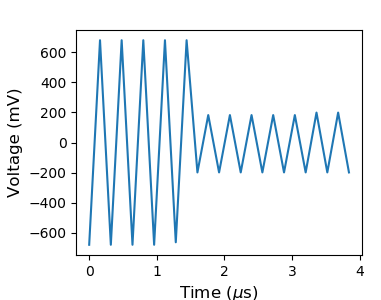
\includegraphics{5-2/pico_bad} %[width=0.3\textwidth]
\caption{The oscilloscope displayed a constant signal throughout the period of data-taking. The data sampled from the pico sampler, however, reconstructs a signal with large aberrations in the first few microseconds.}
\label{fig:pico_start}
\end{figure}

\begin{figure}
\centering
\begin{minipage}{.5\textwidth}
	\centering
	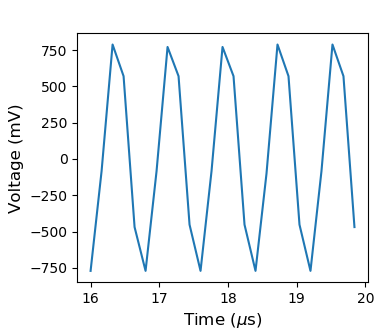
\includegraphics[width=.8\linewidth]{5-2/trial2}
	\caption{$\nu_0 = .2 \nu_s = 1.25$ MHz.}
	\label{fig:Nyq2}
\end{minipage}%
\begin{minipage}{.5\textwidth}
	\centering
	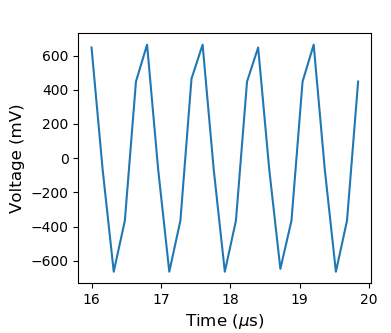
\includegraphics[width=.8\linewidth]{5-2/trial8}
	\caption{$\nu_0 = .8 \nu_s = 5$ MHz.}
	\label{fig:Nyq8}
\end{minipage}
\end{figure}

\begin{figure}
\centering
\begin{minipage}{.5\textwidth}
	\centering
	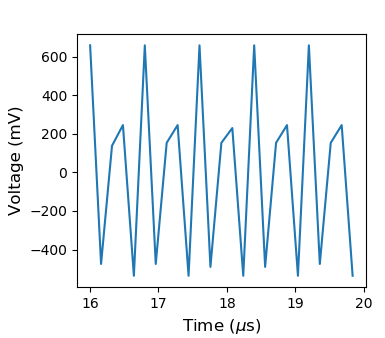
\includegraphics[width=.8\linewidth]{5-2/trial4}
	\caption{$\nu_0 = .4 \nu_s = 2.5$ MHz.}
	\label{fig:Nyq4}
\end{minipage}%
\begin{minipage}{.5\textwidth}
	\centering
	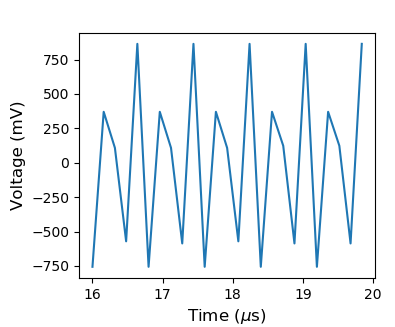
\includegraphics[width=.8\linewidth]{5-2/trial6}
	\caption{$\nu_0 = .6 \nu_s = 3.75$ MHz.}
	\label{fig:Nyq6}
\end{minipage}
\end{figure}
	
\quad We may begin inspection of the samples with a qualitative approach. Figure \ref{fig:Nyq2} shows a signal which repeats about five times in the span of about 4 microseconds. This gives us 1.25 cycles per microsecond, or 1.25 MHz, as expected. Figure \ref{fig:Nyq6} is not as obviously derived from a sine wave (the shape is distorted by the shrinking gap between $\nu_0$ and $\nu_s$), but we may still say that there is a repeating signal with slightly under five repetitions in a span of 4 microseconds. This would give us slighly under 1.25 MHz, which is incorrect; thus we have qualitatively demonstrated an aliasing effect.
% ?? Maybe I should put these annotations in the captions (it would be more appropriate there, I think)

% ?? These figures need annotations. You can probably just do the same qualitative thing that you did before.

\begin{figure}
\centering
\begin{minipage}{.5\textwidth}
	\centering
	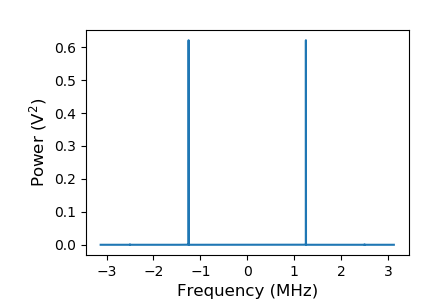
\includegraphics[width=.8\linewidth]{5-2/pow2}
	\caption{$\nu_0 = .2 \nu_s = 1.25$ MHz. Peak amplitudes at $\pm$ 1.25 MHz}
	\label{fig:NyPw2}
\end{minipage}%
\begin{minipage}{.5\textwidth}
	\centering
	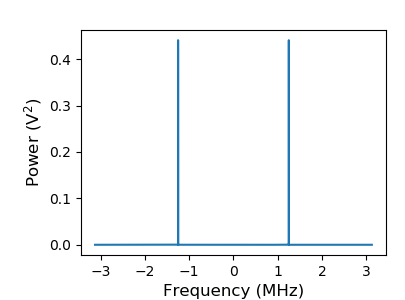
\includegraphics[width=.8\linewidth]{5-2/pow8}
	\caption{$\nu_0 = .8 \nu_s = 5$ MHz. Peak amplitudes at $\pm$ 1.25 MHz}
	\label{fig:NyPw8}
\end{minipage}
\end{figure}

\begin{figure}
\centering
\begin{minipage}{.5\textwidth}
	\centering
	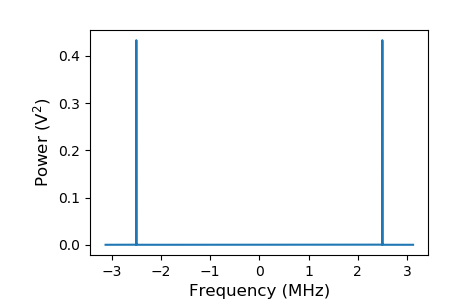
\includegraphics[width=.8\linewidth]{5-2/pow4}
	\caption{$\nu_0 = .4 \nu_s = 2.5$ MHz. Peak amplitudes at $\pm$ 2.5 MHz}
	\label{fig:NyPw4}
\end{minipage}%
\begin{minipage}{.5\textwidth}
	\centering
	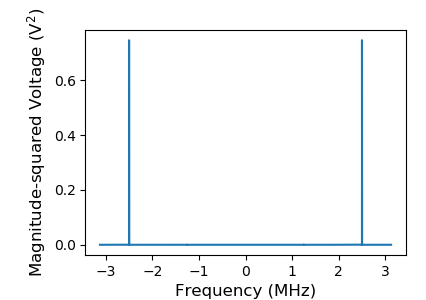
\includegraphics[width=.8\linewidth]{5-2/pow6}
	\caption{$\nu_0 = .6 \nu_s = 3.75$ MHz. Peak amplitudes at $\pm$ 2.5 MHz}
	\label{fig:NyPw6}
\end{minipage}
\end{figure}

\subsection{5.3}

``What does it mean, that the voltage spectra are complex? What do the real and imaginary
parts represent? Is the imaginary part less ‘real’ than the real part? What does it mean, for
frequencies to be negative versus positive?''

``Why might we use power spectra instead of voltage spectra, and vice versa?''

``According to the correlation theorem, the Fourier transform of the power spectrum should equal the ACF. Does it? Explain any differences.''

\

\begin{figure}
\centering
\begin{minipage}{.5\textwidth}
	\centering
	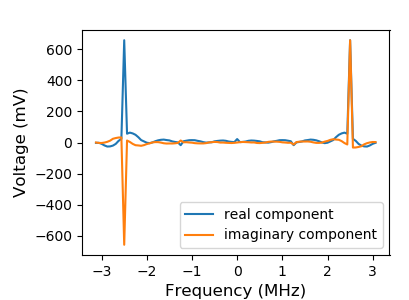
\includegraphics[width=.8\linewidth]{5-3/volt1}
	\caption{Voltage}
	\label{fig:Volt1}
\end{minipage}%
\begin{minipage}{.5\textwidth}
	\centering
	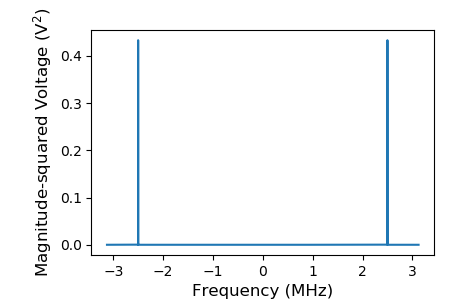
\includegraphics[width=.8\linewidth]{5-3/pow1}
	\caption{Powerish}
	\label{fig:SyPw1}
\end{minipage}
\end{figure}

\begin{figure}
\centering
\begin{minipage}{.5\textwidth}
	\centering
	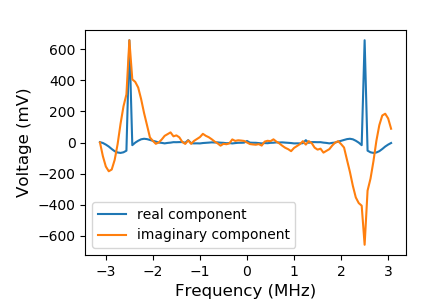
\includegraphics[width=.8\linewidth]{5-3/volt2}
	\caption{Voltage}
	\label{fig:Volt2}
\end{minipage}%
\begin{minipage}{.5\textwidth}
	\centering
	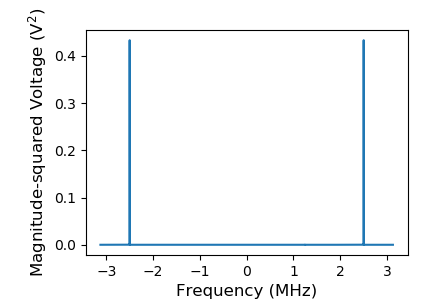
\includegraphics[width=.8\linewidth]{5-3/pow2}
	\caption{Powerish}
	\label{fig:SyPw2}
\end{minipage}
\end{figure}

\begin{figure}
\centering
\begin{minipage}{.5\textwidth}
	\centering
	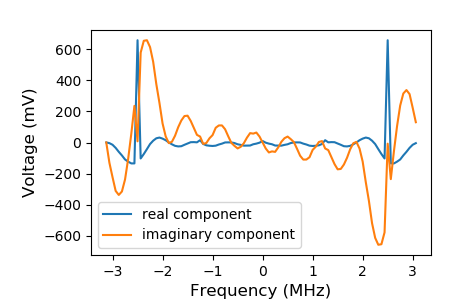
\includegraphics[width=.8\linewidth]{5-3/volt3}
	\caption{Voltage}
	\label{fig:Volt3}
\end{minipage}%
\begin{minipage}{.5\textwidth}
	\centering
	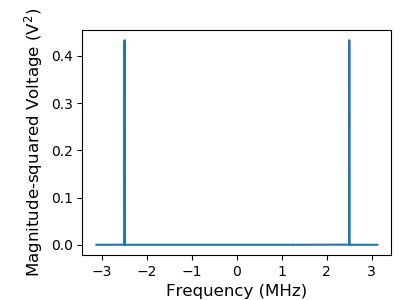
\includegraphics[width=.8\linewidth]{5-3/pow3}
	\caption{Powerish}
	\label{fig:SyPw3}
\end{minipage}
\end{figure}

``you need to make sure dft.idft correctly infers the frequencies corresponding to each bins in your power spectrum array''

``When calculating a digital version of the correlation function, you have to worry about end effects.
Suppose you are calculating an ACF for N samples with delays ∆N ranging up to N/2. Then the
number of terms in the sum is always smaller than N because the delays spill over the edge of the
available samples.''

\textcolor{red}{How am I supposed to account for this?}

\begin{figure}
\centering
\begin{minipage}{.5\textwidth}
	\centering
	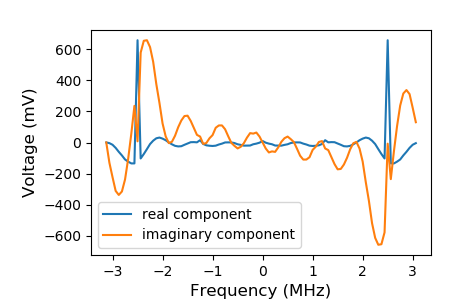
\includegraphics[width=.8\linewidth]{5-3/volt3}
	\caption{Voltage}
	\label{fig:inverse}
\end{minipage}%
\begin{minipage}{.5\textwidth}
	\centering
	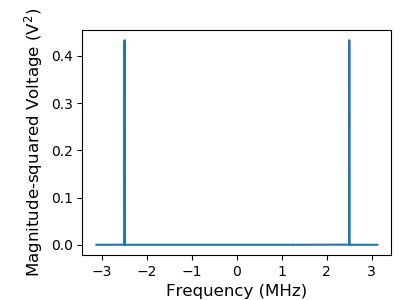
\includegraphics[width=.8\linewidth]{5-3/pow3}
	\caption{Powerish}
	\label{fig:ACF}
\end{minipage}
\end{figure}

\textcolor{red}{Differences? Probably because I did not zero out the middle}

\subsection{5.4}

\begin{figure}
\centering
\begin{minipage}{.5\textwidth}
	\centering
	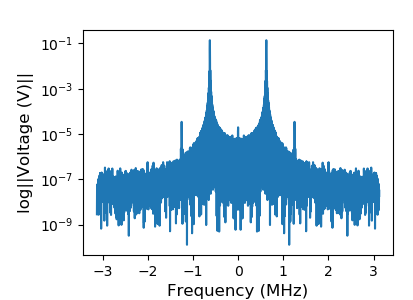
\includegraphics[width=.8\linewidth]{5-4/t1_quarter}
	\caption{$\nu_0 = .1 \nu_s = .625$ MHz}
	\label{fig:tenth_leakage}
\end{minipage}%
\begin{minipage}{.5\textwidth}
	\centering
	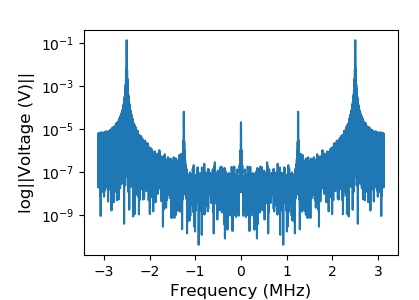
\includegraphics[width=.8\linewidth]{5-4/t4_quarter}
	\caption{$\nu_0 = .4 \nu_s = 2.5$ MHz}
	\label{fig:4tenths_leakage}
\end{minipage}
\end{figure}

\textcolor{red}{The y-axis is labeled incorrectly. We want log of square of voltage.}

Recall that spectral leakage is introduced by the finite bounds on our Fourier transforms. Why does that math correspond to these results?

\subsection{5.5}

\textcolor{red}{The separation looks pretty good so far.}

\subsection{5.6}

\begin{figure}
\centering
\begin{minipage}{.5\textwidth}
	\centering
	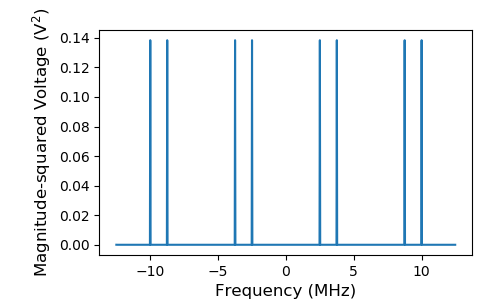
\includegraphics[width=.9\linewidth]{5-6/4window}
	\caption{$\nu_0 = .4 \nu_s = 2.5$ MHz. Fourth window.}
	\label{fig:win4}
\end{minipage}%
\begin{minipage}{.5\textwidth}
	\centering
	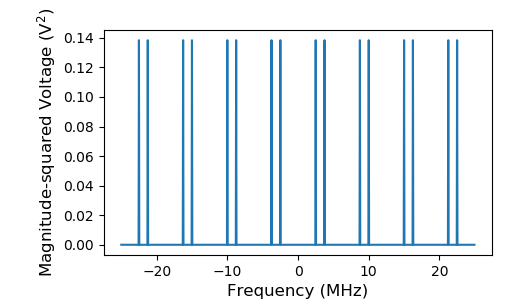
\includegraphics[width=.9\linewidth]{5-6/8window}
	\caption{Same frequency. Eighth window.}
	\label{fig:win8}
\end{minipage}
\end{figure}

\begin{figure}
\centering
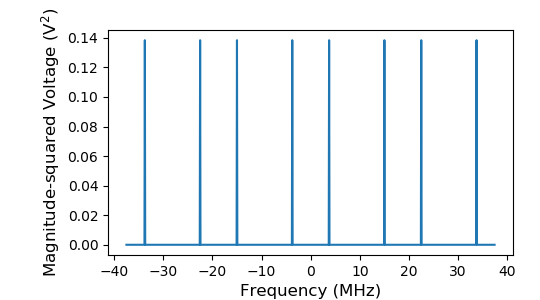
\includegraphics[width=.45\linewidth]{5-6/12window}
\caption{Same frequency. Twelth window.}
\label{fig:win12}
\end{figure}

% They can't be harmonics; why else would all the spikes have the same amplitudes. And, for that matter, why do all windows show such low amplitudes? Ah, it is because the input signal (as seen on the oscilloscope) has a much lower amplitude--squaring further affects to that end.

\subsection{5.7}

First sample:

Mean = 3.899292452830189 mV
Standard deviation = 20.079642416978363 mV
Variance = 403.19203959371663 (mV)$^2$

\textcolor{red}{I am allowing the first 100 samples to contaminate. I do not know how much I should trod outside the 16000 recommendation.}

\begin{figure}
\centering
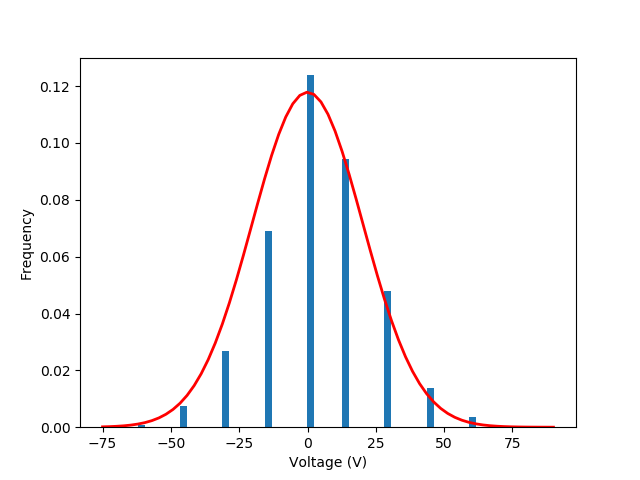
\includegraphics[width=.45\linewidth]{5-7/histo}
\caption{}
\label{fig:histogram}
\end{figure}

\begin{figure}
\centering
\begin{minipage}{.5\textwidth}
	\centering
	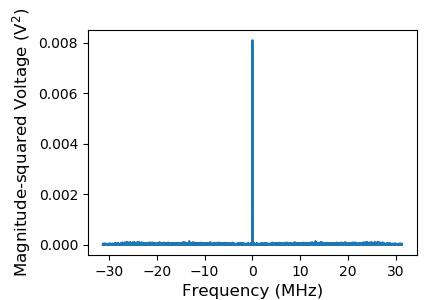
\includegraphics[width=.9\linewidth]{5-7/pow1}
	\caption{}
	\label{fig:pow1}
\end{minipage}%
\begin{minipage}{.5\textwidth}
	\centering
	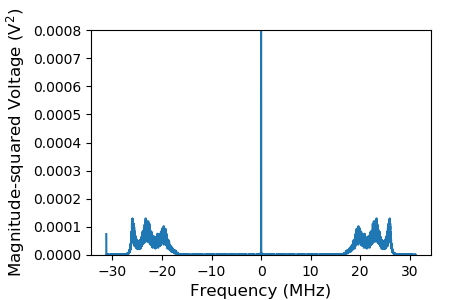
\includegraphics[width=.9\linewidth]{5-7/pow_all}
	\caption{}
	\label{fig:pow_all}
\end{minipage}
\end{figure}

\begin{figure}
\centering
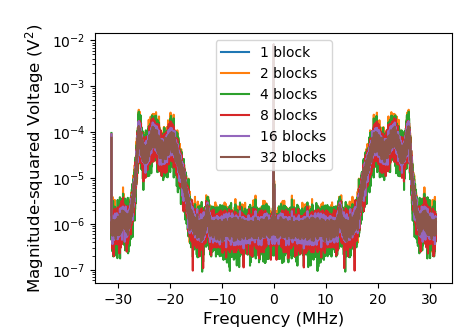
\includegraphics[width=\linewidth]{5-7/comparison}
\caption{}
\label{fig:avgs_comparison}
\end{figure}

\subsection{7.1}

\begin{figure}
\centering
\begin{minipage}{.5\textwidth}
	\centering
	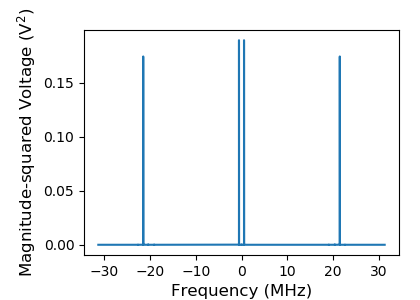
\includegraphics[width=.8\linewidth]{7-1/l_power}
	\caption{}
	\label{fig:low_pow}
\end{minipage}%
\begin{minipage}{.5\textwidth}
	\centering
	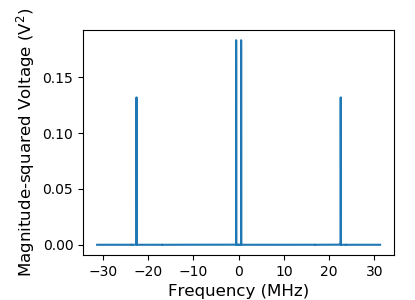
\includegraphics[width=.8\linewidth]{7-1/h_power}
	\caption{}
	\label{fig:high_pow}
\end{minipage}
\end{figure}

\begin{figure}
\centering
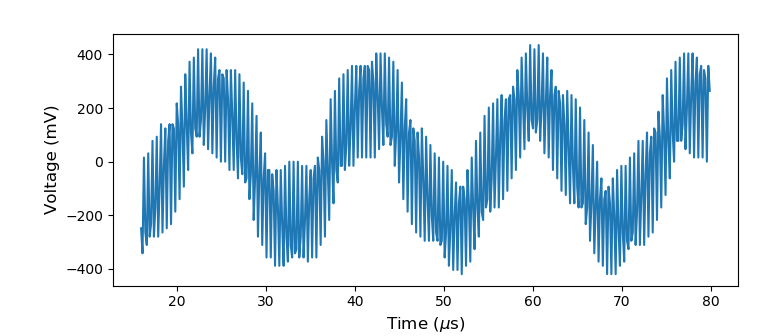
\includegraphics[width=.45\linewidth]{7-1/low_osc}
\caption{}
\label{fig:low_display}
\end{figure}

\textcolor{red}{These figures are missing captions!}

\subsection{7.2}

\subsection{7.3}

% I really do not want to take this data, so I am deliberately leaving a more challenging analysis task for last-minute

Single side band mixer is more difficult to perform.

\section{Conclusions}

\bibliographystyle{alpha}
\bibliography{sample}

\end{document}